\section{Aperture Antennas}
\subsection{Rectangular Apertures, Horn Antennas}
\begin{itemize}
    \itemsep0pt
    \item \textbf{Fundamental mode:} $\mathrm{TE}_{10}$ ($\mathrm{H_{10}}$)
        \begin{equation*}
            \beta = \sqrt{k^2 - k_c^2} = \sqrt{k^2 -\left(\dfrac{m\pi}{A}\right)^2 -\left(\dfrac{n\pi}{B}\right)^2}
        \end{equation*}
    \item $\mathrm{H}_{10}$-mode of a rectangular waveguide with the origin in its aperture:
        \begin{center}
            \begin{tikzpicture}[
        scale=1.0,
        transform shape,
        >=Stealth,
        dotarrow/.style={circle,draw,inner sep=0pt,minimum size=.3cm,path picture={
        \fill (0,0) circle[radius=.6mm];}, node contents={}}]
    % Coordinates and aperture
    \path (0,0) node(O)[dotarrow];
    \draw[-{>[length=3mm, width=2mm]}] (O) -- (0, 1)node[left]{$y$};
    \draw[-{>[length=3mm, width=2mm]}] (O) -- (1, 0)node[below]{$x$};
    \draw node[below left] at (O){$z$};
    \draw[very thick] (O) rectangle (4, 2);
    % E-field
    \draw (O) sin (2, 1) (4,0) sin (2, 1);
    \foreach \x in {.5, 1, ..., 3.5}{
        \pgfmathsetmacro{\mylen}{sin((pi/4)*\x r)}
        \draw[red, ->] (\x, 0) -- (\x, \mylen);
    }
    % H-field
    \foreach \y in {1.2, 1.5, 1.8}{
        \draw[thin, blue, ->] (0, \y) -- (.5, \y);
        \draw[blue, ->] (.5, \y) -- (1.25, \y);
        \draw[blue, ->] (1.25, \y) -- (2.75, \y);
        \draw[blue, ->] (2.75, \y) -- (3.5, \y);
        \draw[very thin, blue, ->] (3.5, \y) -- (4, \y);
    }
    %% Legend
    %\path (4.9, 1.5)node[circle, fill=blue!]{} (5, 1.5) node[right]{$\vec{H}$};
    %\path (4.9, 1)node[circle, fill=red!]{} (5, 1) node[right]{$\vec{E}$};
    % Measurements
    \draw[{Bar}{Stealth}-{Stealth}{Bar}] (0, -.4) --node[below]{$A$, $m=1$} (4, -.4);
    \draw[{Bar}{Stealth}-{Stealth}{Bar}] (4.2, 2) --node[right]{$B$, $n=0$} (4.2, 0);
\end{tikzpicture}

        \end{center}
        \begin{align*}
            &E_y = E_0 \sin\left(\dfrac{\pi}{A}x\right) e^{-j\beta z},\\
            &H_x = -\dfrac{E_y}{Z_{FH}} = -\dfrac{E_y}{Z_{F0}} \sqrt{1 - \left(\dfrac{\lambda_0}{2A}\right)^2} e^{-j\beta z},\\
            &H_z = j \dfrac{E_0}{Z_{F0}} \dfrac{\lambda_0}{\lambda_c} \cos\left(\dfrac{\pi}{a}x\right) e^{-j\beta z},\\
            &Z_{FH} = \dfrac{\mu\epsilon}{\beta} = \frac{\lambda_g}{\lambda_0} Z_{F0}
        \end{align*}
    \item Radiation pattern is obtained by \textit{Fourier Transform of aperture distribution}.
    \item \textbf{Far-field of Rectangular Aperture} with uniform field distribution:
        \begin{align*}
            E_{\vartheta} &= -jE_0 \dfrac{AB}{\lambda} \dfrac{e^{-jkr}}{r} C(\vartheta, \varphi),\\
            C(\vartheta, \varphi) &= \cos\varphi\
            \mathrm{si}\left(\pi \dfrac{A}{\lambda}\sin\varphi\sin\vartheta\right)\
            \mathrm{si}\left(\pi \dfrac{B}{\lambda}\cos\vartheta\right),\\
            \text{\textit{With: }}&\mathrm{si}(x) = \dfrac{\sin(x)}{x}
        \end{align*}
    \item Half power beam width (HPBW):
        \begin{align*}
            &\text{H-Plane, } \vartheta = \dfrac{\pi}{2} \text{:}\
            &\dfrac{\varphi_{\SI{3}{dB}}}{\mathrm{deg}} \approx 50.4 \dfrac{\lambda}{A}\\
            &\text{E-Plane, } \varphi = 0 \text{:}\
            &\dfrac{\vartheta^\prime_{\SI{3}{dB}}}{\mathrm{deg}} \approx 50.4 \dfrac{\lambda}{B}
        \end{align*}
            \(\implies \text{Side-lobe: } a_{SL} = 20 \log \dfrac{1}{0.21} \approx \SI{13.6}{dB}\)
    \item Directivity $D$ of \textit{rectangular aperture}:
        \begin{equation*}
            D = \left(\dfrac{S_{\mathrm{max}}}{S_I}\right)_{P_t} = \dfrac{(AB)^2 4\pi r^2}{\lambda^2 r^2 AB} = 4\pi \dfrac{AB}{\lambda^2}
        \end{equation*}
    \item \textbf{Horn of infinite length:}
        \begin{align*}
            E_z &= E_0 \cos\left(\dfrac{\pi y}{A}\right),\\
            E_{\vartheta} &= -jE_0 \dfrac{AB}{\lambda} \dfrac{2}{\pi} \dfrac{e^{-jkr}}{r} C(\vartheta, \varphi),\\
            C(\vartheta, \varphi) &= \cos\varphi\
            \dfrac{\cos\left(\pi \frac{A}{\lambda}\sin\varphi\sin\vartheta\right)}{1 - \left(2 \frac{A}{\lambda}\sin\varphi\sin\vartheta\right)^2}\
            \mathrm{si}\left(\pi \dfrac{A}{\lambda}\cos\vartheta\right)
        \end{align*}
    \item Directivity D of \textit{Horn of infinite extent:}\\
        \(D = \dfrac{4\pi}{\lambda^2}qAB,\;\;q \text{: aperture efficiency}\)
    \item Horns of finite extent:
        \begin{itemize}
            \itemsep0pt
            \item E-plane horn: \(B>b\),
            \item H-plane horn: \(A>a\),
            \item Pyramidal horn: \(B>b \text{ and  } A>a\)
        \end{itemize}
\end{itemize}

\subsection{Corrugated Horns}
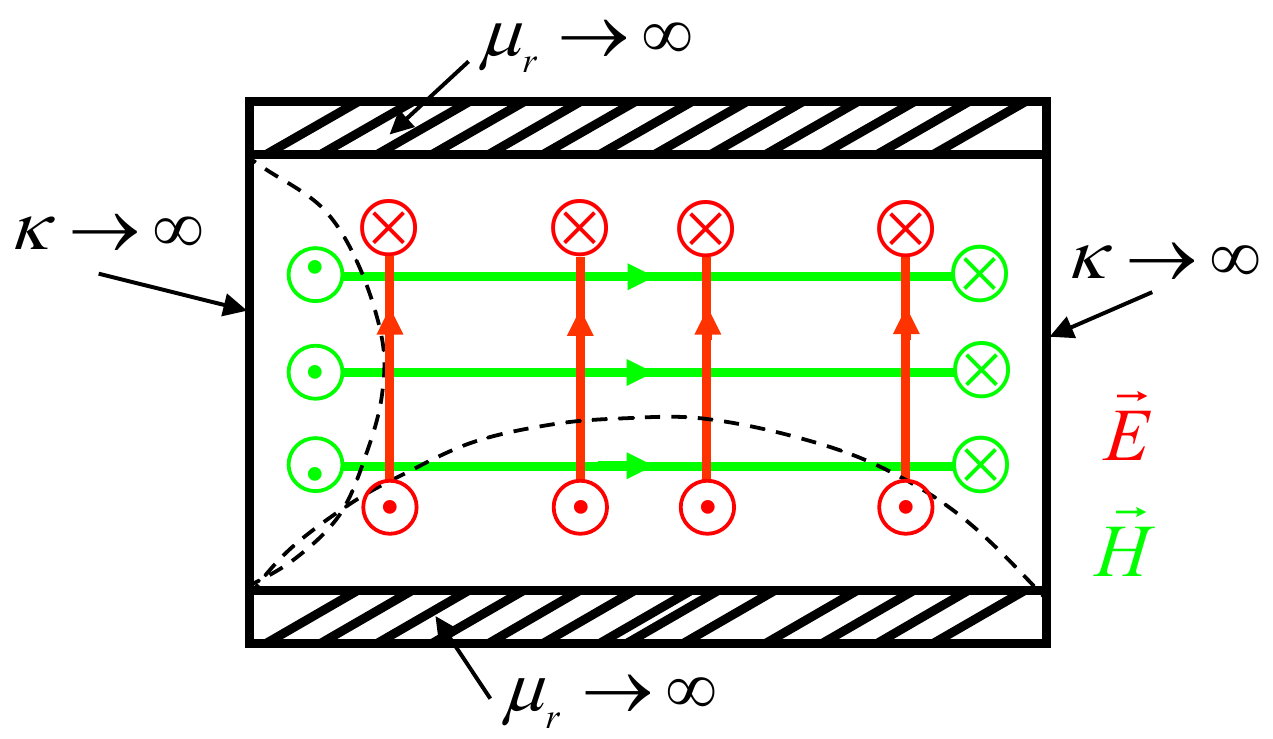
\includegraphics[width=4.5cm]{content/aawp/pictures/corrugated_horn_magn_walls.png}
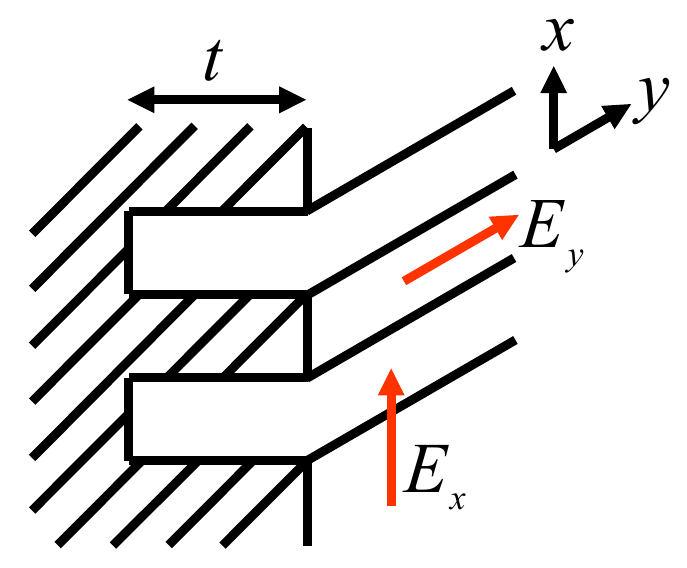
\includegraphics[width=3cm]{content/aawp/pictures/corrugated_wall.png}
\begin{itemize}
    \itemsep0pt
    \item \textbf{Design Goal:} Taper of the aperture field distribution in $E$-plane as well
    \item Anisotropic surface impedance (grooved walls):
        \begin{align*}
            &\text{For }E_\parallel: \quad Z_{S\parallel} = 0,\\
            &\text{For }E_\perp:     \quad Z_{S\perp} \to \infty
        \end{align*}
    \item Corrugations \textit{improve} sidelobe and forward/backward behaviour
    \item $E$- and $H$-plane patterns become more similar
\end{itemize}

\subsection{Circular Aperture}
\begin{center}
    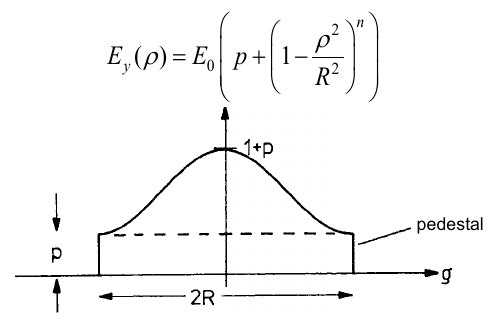
\includegraphics[width=.3\paperheight]{content/aawp/pictures/circular_aperture_distribution.png}
\end{center}
\begin{align*}
    %\text{For:} \quad &E(\rho) = E_0 \left(p + \left(1 - \dfrac{\rho^2}{R^2}\right)^n\right)\\\\
    \implies &E_y = \left(p + \dfrac{1}{n+1}\right) \dfrac{jE_0 k R^2}{2} \dfrac{e^{jkr}}{r}C(\vartheta),\\
    C(\vartheta) &= \dfrac{1}{p + \frac{1}{1+n}}\
    \left(\dfrac{J_1(\xi)}{\xi/2} + \dfrac{n!\,J_{n+1}(\xi)}{(\xi/2)^{n+1}}\right),\\
    \xi = &kR\sin\vartheta,\\
    J_\alpha:&\text{ Bessel function, first kind}
\end{align*}
\textbf{Aperture efficiency} (of cicular aperture):
\begin{equation*}
    q_a = \dfrac{A_{\mathrm{eff}}}{A_{\mathrm{geo}}} = \dfrac{\left[p + \dfrac{1}{n+1}\right]^2}{p^2 + \dfrac{2p}{n+1} + \dfrac{1}{2n+1}}
\end{equation*}
\textbf{Consider uniform field distribution} (\(p=0, n=0\)):
\begin{equation*}
    C(\vartheta) = 2\dfrac{J_1(kR\sin(\vartheta))}{kR\sin\vartheta} = 2\dfrac{J_1(\pi u)}{\pi u}, \quad u = \dfrac{2R}{\lambda}\sin\vartheta
\end{equation*}
\begin{equation*}
    \implies \dfrac{\vartheta_{\SI{3}{dB}}}{\mathrm{deg}} \approx 57\dfrac{\lambda}{2R}, \quad a_{\mathrm{SL}} \approx \SI{17.7}{dB}
\end{equation*}

\subsection{Reflector Antennas}
\begin{tabular}{cc}
    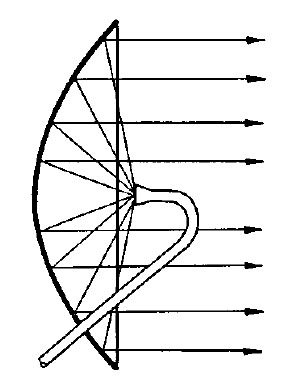
\includegraphics[width=3cm]{content/aawp/pictures/parabolic_reflector_antenna.png}
    &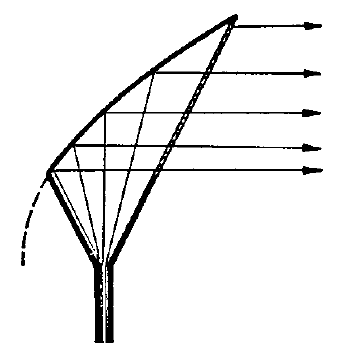
\includegraphics[width=4cm]{content/aawp/pictures/hyperbolic_reflector_antenna.png}\\
    \textbf{Parabolic Dish} & \textbf{Hyperbolic Dish}
\end{tabular}
\begin{itemize}
    \itemsep0pt
    \item \textbf{Goal:} In-phase illumination of a \textit{large aperture}
    \item Point source in focues of parabola generates planar wavefront
    \item \textit{High gain/directivity} antennas
    \item Common refelctor shapes (\textit{conic sections}):
        \begin{itemize}
            \itemsep0pt
%            \item Ellipsoid(?)
            \item Paraboloid (e.g. radio telescope)
            \item Hyperboloid (e.g. TV antenna) $\to$ off-axis feed
            \item Cassegrain: two reflectors, \textit{convex} secondary refelctor
            \item Gregorian: two reflectors, \textit{concave} secondary refelctor
        \end{itemize}
    \item Treatment using \textbf{Physical Optics}: field distribution on reflector using ray optics, far-field using Huygen's principle on reflector:
        \begin{align*}
            &\vec{J}_A = 0 &\text{in \textit{shadow} region}\\
            &\vec{J}_A = 2\vec{n} \times\vec{H}^{\mathrm{inc}}(0) &\text{in \textit{lit} region}\\
            &\vec{M}_A = -\vec{n}\times\vec{E} = 0
        \end{align*}
\end{itemize}
\subsection{Lens Antennas}
\begin{itemize}
    \item Concave \textit{delay lens} with $\epsilon_r > 1$
    \item Convex \textit{fast lens} with $\epsilon_r < 1$
    \item Spherical \textit{Luneberg lens} with concentric $\epsilon_r$ gradient
    \item \textit{Einstein gravity lens}  $\implies$ General relativity warps spacetime around celestial body; EM-waves are bent around celestial body
\end{itemize}
